\documentclass[aspectratio=43]{beamer}
% vim: nospell
\usepackage{bibentry}
\usepackage{booktabs}
\usepackage{xspace}
\usepackage{listings}
\hypersetup{draft}
\usepackage{tikz}

\usepackage{GoSans}
\usepackage{GoMono}
\usepackage{fourier}
%\usepackage{arev}
\usepackage[T1]{fontenc}
%\usefonttheme{serif}
\usefonttheme[onlymath]{serif}

\usecolortheme{beetle}
\setbeamercolor{structure}{bg=beetle@other}
\setbeamercolor{block body}{bg=black!20}

%\usecolortheme{orchid}
%\usecolortheme{whale}

%\useoutertheme{infolines}
%\setbeamertemplate{headline}{}
\setbeamertemplate{navigation symbols}{}
\addtobeamertemplate{navigation symbols}{}{%
    \usebeamerfont{footline}%
    \usebeamercolor[black]{}%
    \insertframenumber/\inserttotalframenumber
}
%\useinnertheme[shadow]{rounded}
%\setbeamertemplate{items}[triangle]
%\useinnertheme{circles}
\useinnertheme{rectangles}

\setbeamercovered{transparent}

\newcommand{\sectiontoc}[1]{
    \section{#1}
    \begin{frame}%{Outline}
    \tableofcontents[currentsection]
    \end{frame}
}

\newcommand{\subsectiontoc}[1]{
    \subsection{#1}
    \begin{frame}%{Outline}
    \tableofcontents[currentsubsection]
    \end{frame}
}

\newcommand{\R}{\mathbb{R}}

\begin{document}

\title{convGEMM}

% \author{%
% Jos\'e~I.~Aliaga\inst{1}
% \and
% Hartwig~Anzt\inst{2,3}
% \and
% Enrique~S.~Quintana-Ort\'{\i}\inst{4}
% \and
% \textbf{Andr\'es~E.~Tom\'as}\inst{1,5}
% \and
% Yuhsiang M. Tsai\inst{2}
% }
% %\authorrunning{J. I. Aliaga et al.}
% 
% \institute{%
% Dpto. d'Enginyeria i Ci\`encia dels Computadors, Universitat Jaume I, Spain
% \and
% Steinbuch Centre for Computing, Karlsruhe Institute of Technology, Germany
% \and
% Innovative Computing Lab, University of Tennessee, USA
% \and
% DISCA, Universitat Polit\`ecnica de Val\`encia, Spain
% \and
% Dpto. de Inform\'atica, Universitat de Val\`encia, Spain
% }

\date{8 septiembre 2021}

\begin{frame}%[plain]
\titlepage
\end{frame}

% \begin{frame}{Outline}
% \tableofcontents
% \end{frame}

\begin{frame}{Redes neuronales convolucionales}
La red neuronal es convolucional, el convolucionador que la convolucione buen convolucionador será.
\end{frame}

\begin{frame}{Convolución usando la GEMM}

\begin{block}{Formato NCHW}
\begin{description}
    \item[Forward] out = trans12(im2col(image) * kernel + bias)
    \item[Backward]
    \begin{enumerate}
        \item kernel = trans(im2col(image)) * trans12(out)
        \item image = col2im(trans(12(out)) * kernel)
    \end{enumerate}
\end{description}
\end{block}

\begin{block}{Formato NHWC}
\begin{description}
    \item[Forward] out = kernel * im2row(image) + bias
    \item[Backward]
    \begin{enumerate}
        \item kernel = out * trans(im2row(image))
        \item image = row2im(kernel * out)
    \end{enumerate}
\end{description}
\end{block}

\begin{description}
    \item[Problema:] se necesita mucha memoria para las matrices intermedias

    \item[Solución:] usar la GEMM de BLIS sin construir las matrices intermedias
\end{description}

\end{frame}

\begin{frame}%[plain]
    \begin{tikzpicture}[remember picture,overlay]
        \node[at=(current page.center)] {
            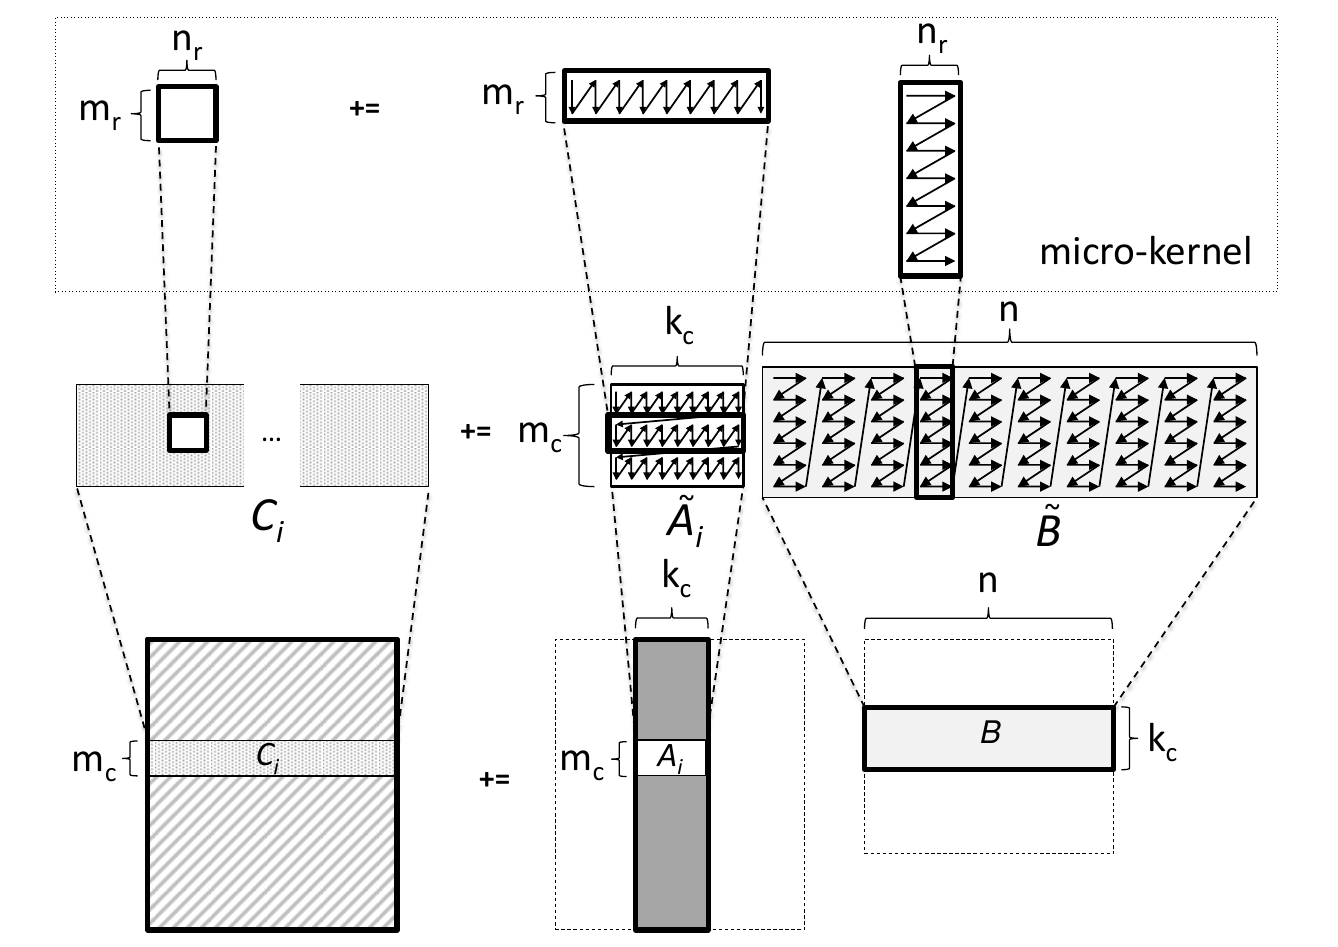
\includegraphics[height=\paperheight]{blis.png}
        };
    \end{tikzpicture}
\end{frame}

\begin{frame}%[plain]
    \begin{tikzpicture}[remember picture,overlay]
        \node[at=(current page.center)] {
            \includegraphics[width=\paperwidth]{../plots/blas-volta.pdf}
        };
    \end{tikzpicture}
\end{frame}

\begin{frame}[fragile]{Parámetros BLIS}
\begin{lstlisting}[language=C,basicstyle=\scriptsize\ttfamily]
bli_init();

cntx_t* cntx = bli_gks_query_cntx();

sgemm_ukr_ft gemm_kernel =
    bli_cntx_get_l3_nat_ukr_dt(BLIS_FLOAT, BLIS_GEMM, cntx);

MR = bli_cntx_get_blksz_def_dt(BLIS_FLOAT, BLIS_MR, cntx); // 32
NR = bli_cntx_get_blksz_def_dt(BLIS_FLOAT, BLIS_NR, cntx); // 12
MC = bli_cntx_get_blksz_def_dt(BLIS_FLOAT, BLIS_MC, cntx); // 480
NC = bli_cntx_get_blksz_def_dt(BLIS_FLOAT, BLIS_NC, cntx); // 3072
KC = bli_cntx_get_blksz_def_dt(BLIS_FLOAT, BLIS_KC, cntx); // 384

float *Ac = aligned_alloc(4096, MC * KC * sizeof(float));
float *Bc = aligned_alloc(4096, KC * NC * sizeof(float));
float *Csmall = aligned_alloc(4096, MR * NR * sizeof(float));
float *Cbig   = aligned_alloc(4096, MC * NC * sizeof(float));
\end{lstlisting}
% kernel = 0x7f2cd0a79b60 MR = 32 NR = 12 packmr = 32 packnr = 12 row_pref = 0 NC = 3072 MC = 480 KC = 384
\end{frame}

\begin{frame}%[plain]
    \begin{tikzpicture}[remember picture,overlay]
        \node[at=(current page.center)] {
            \includegraphics[width=\paperwidth]{../plots/blis-volta.pdf}
        };
    \end{tikzpicture}
\end{frame}

\begin{frame}[fragile]{Nuevo interfaz GEMM}
\begin{lstlisting}[language=C,basicstyle=\scriptsize\ttfamily]
void gemm_blis_B3A2C0(char orderA, char orderB, char orderC,
                      char transA, char transB,
                      int m, int n, int k,
                      float alpha, const float *A, int ldA,
                      const float *B, int ldB,
                      float beta, float *C, int ldC,
                      float *Ac, pack_func pack_RB,
                      float *Bc, pack_func pack_CB,
                      float *Cc, post_func postprocess,
                      cntx_t *cntx, const convol_dim *dim,
                      const float *bias_vector)

typedef struct {
    int batch, height, width, channel, kn, kheight, kwidth,
    vstride, hstride, vpadding, hpadding, vdilation, hdilation,
    oheight, owidth;
} convol_dim;
\end{lstlisting}
\end{frame}

\begin{frame}[fragile]{Funciones de empaquetado y postproceso}
\begin{lstlisting}[language=C,basicstyle=\scriptsize\ttfamily]
typedef void (*pack_func)(char orderM, char transM, int mc, int nc,
                          const float *M, int ldM, float *Mc, int RR,
                          const convol_dim *dim,
                          int start_row, int start_col);

typedef void (*post_func)(int mr, int nr, const float *Cc, int ldCc,
                          float beta, float *C, int ldC,
                          const convol_dim *dim,
                          const float *bias_vector,
                          int start_row, int start_col, bool last);
\end{lstlisting}
\end{frame}

\begin{frame}[fragile]{Operaciones para NCHW}
\begin{lstlisting}[language=C,basicstyle=\scriptsize\ttfamily]
gemm_blis_B3A2C0('C', 'C', 'C', 'N', 'N',
                 ho * wo * b, kn, kh * kw * c,
                 alpha, image, ho * wo * b, kernel, kh * kw * c,
                 beta, out, ho * wo * b,
                 ac_pack, pack_RB_nchw, bc_pack, pack_CB,
                 cc_pack, add_bias_transpose_nchw,
                 cntx, &dim, bias_vector);

gemm_blis_B3A2C0('C', 'C', 'C', 'T', 'N',
                 kh * kw * c, kn, ho * wo * b,
                 alpha, image, ho * wo * b, out, ho * wo * b,
                 beta, kernel, kh * kw * c,
                 ac_pack, pack_RB_nchw, bc_pack, pack_CB_nchw_trans,
                 cc_pack, NULL,
                 cntx, &dim, NULL);

gemm_blis_B3A2C0('C', 'C', 'C', 'N', 'T',
                 b * ho * wo, c * kh * kw, kn,
                 alpha, out, b * ho * wo, kernel,
                 c * kh * kw, 1.0, image, b * ho * wo,
                 ac_pack, pack_RB_nchw_trans, bc_pack, pack_CB,
                 cc_pack, post_col2im_nchw,
                 cntx, &dim, NULL);
\end{lstlisting}
\end{frame}

% \subsectiontoc{NCHW}

\begin{frame}%[plain]
    \begin{tikzpicture}[remember picture,overlay]
        \node[at=(current page.center)] {
            \includegraphics[width=\paperwidth]{../plots/convgemm_nchw-volta.pdf}
        };
    \end{tikzpicture}
\end{frame}

\begin{frame}%[plain]
    \begin{tikzpicture}[remember picture,overlay]
        \node[at=(current page.center)] {
            \includegraphics[width=\paperwidth]{../plots/trans_nchw-volta.pdf}
        };
    \end{tikzpicture}
\end{frame}

\begin{frame}%[plain]
    \begin{tikzpicture}[remember picture,overlay]
        \node[at=(current page.center)] {
            \includegraphics[width=\paperwidth]{../plots/back_nchw-volta.pdf}
        };
    \end{tikzpicture}
\end{frame}

% \subsectiontoc{NHWC}

\begin{frame}[fragile]{Operaciones para NHWC}
\begin{lstlisting}[language=C,basicstyle=\scriptsize\ttfamily]
gemm_blis_B3A2C0('C', 'C', 'C', 'N', 'N',
                 kn, ho * wo * b, kh * kw * c,
                 alpha, kernel, kn, image, kh * kw * c,
                 beta, out, kn,
                 ac_pack, pack_RB, bc_pack, pack_CB_nhwc,
                 cc_pack, add_bias_nhwc,
                 cntx, &dim, bias_vector);

gemm_blis_B3A2C0('C', 'C', 'C', 'N', 'T',
                 kn, kh * kw * c, ho * wo * b,
                 alpha, out, kn, image, kh * kw * c,
                 beta, kernel, kn,
                 ac_pack, pack_RB, bc_pack, pack_CB_nhwc,
                 cc_pack, NULL,
                 cntx, &dim, NULL);

gemm_blis_B3A2C0('C', 'C', 'C', 'T', 'N',
                 c * kh * kw, ho * wo * b, kn,
                 alpha, kernel, kn, out, kn,
                 1.0, image, c * kh * kw,
                 ac_pack, pack_RB, bc_pack, pack_CB,
                 cc_pack, post_row2im_nhwc,
                 cntx, &dim, NULL);
\end{lstlisting}
\end{frame}

\begin{frame}%[plain]
    \begin{tikzpicture}[remember picture,overlay]
        \node[at=(current page.center)] {
            \includegraphics[width=\paperwidth]{../plots/convgemm-volta.pdf}
        };
    \end{tikzpicture}
\end{frame}

\begin{frame}%[plain]
    \begin{tikzpicture}[remember picture,overlay]
        \node[at=(current page.center)] {
            \includegraphics[width=\paperwidth]{../plots/trans-volta.pdf}
        };
    \end{tikzpicture}
\end{frame}

\begin{frame}%[plain]
    \begin{tikzpicture}[remember picture,overlay]
        \node[at=(current page.center)] {
            \includegraphics[width=\paperwidth]{../plots/back-volta.pdf}
        };
    \end{tikzpicture}
\end{frame}

\begin{frame}
    \begin{block}{Trabajo hecho}
    \begin{itemize}
        \item Padding implícito
        \item Cualquier combinación de \emph{stride}, \emph{padding} y \emph{dilation}
        \item Formatos NCHW y NHWC
        \item Independiente de la arquitectura
        \item B3A2A0 y A3B2C0
        \item Bias y transposición dentro de GEMM
        \item Simplificación código Python
    \end{itemize}
    \end{block}

    \begin{block}{Por hacer}
    \begin{itemize}
        \item Usar buffer pequeño para biases y trans. NCHW
        \item Añadir activaciones al postproceso
        \item Quitar condiciones de carrera en la deconvolución
        \item Gestión de memoria en Python
    \end{itemize}
    \end{block}
\end{frame}

\end{document}
